% Template for ApJ-type papers

\documentclass[12pt,preprint]
%{aastex}
{emulateapj}

\usepackage{rotating}
\usepackage{amssymb,amsmath}
%\usepackage{graphicx}[subfloat]
\usepackage{multirow}
\citestyle{aa}

\bibliographystyle{apj_w_etal}

\newcommand{\vect}[1]{\mathbf{#1}}
\newcommand{\xad}{\vect{x}}

\newcommand{\vdag}{(v)^\dagger}
\newcommand{\myemail}{jaguirre@nrao.edu}
\newcommand{\lsim}{{_{<}\atop^{\sim}}}
\newcommand{\gsim}{{_{>}\atop^{\sim}}}
\newcommand{\etal}{{et al.\/}}
\newcommand{\ie}{{\em ie.\/}}
\newcommand{\cmq}{cm{$^{-3}$}}
\newcommand{\per}{$^{\rm{-1}}$}
\newcommand{\tc}{{$\theta^1$~Orionis~C}}
%\newcommand{\msol}{M{$_{\odot}$}}
\def\msol{\ifmmode {\>M_\odot}\else {$M_\odot$}\fi}
\newcommand{\lsol}{L{$_{\odot}$}}
\newcommand{\kms}{km~s{$^{-1}$}}
\newcommand{\hii}{H~{\sc ii}}
\newcommand{\Hii}{H~{\sc ii}}
\newcommand{\Ha}{\mbox{H$\alpha$}}
\newcommand{\sii}{S~{\sc ii}}
\newcommand{\Feii}{Fe~{\sc ii}}
\newcommand{\oi}{O~{\sc i}}
\newcommand{\nii}{N~{\sc ii}}
\newcommand{\oiii}{O~{\sc iii}}
\newcommand{\mgii}{Mg~{\sc ii}}
\newcommand{\tco}{{$^{13}$CO}}
\newcommand{\CO}{{$^{12}$CO}}
\newcommand{\Tco}{{$^{12}$CO}}
\newcommand{\co}{C{$^{18}$O}}
\newcommand{\Lsol}{L$_{\odot}$}
\newcommand{\Msol}{M$_{\odot}$}
%\newcommand{\C18o}{C$^{18}$O($1\rightarrow 0$)}
\newcommand{\Check}{{\bf ???}}
\newcommand{\mum}{\ensuremath{\mu \mathrm{m}}}
\newcommand{\flux}{flux density}
\newcommand{\solar}{\ensuremath{\odot}}

\newcommand{\epsi}{\varepsilon}
\newcommand{\herschel}{{\em Herschel}}


\newcommand{\TBD}{{\bf TBD}}

\def\Figure#1#2#3#4{
\begin{figure}[htb]
\epsscale{#4}
\plotone{#1}
\caption{#2}
\label{#3}
\end{figure}
}

\def\Table#1#2#3#4#5{
\begin{deluxetable}{#1}
\tablewidth{0pt}
\tablecaption{#2}
\tablehead{#3}
\startdata
\label{#4}
#5
\enddata
\end{deluxetable}
}

\newcommand{\cii}{[C{\sc ii}]}
\def\hi{H{\sc i}}
\newcommand{\smg}{SMG}
\newcommand{\smgs}{SMGs}

\newcommand{\penn}{1}
\newcommand{\jpl}{2}
	% End definitions


\shorttitle{Measuring galaxy clustering with Far-IR line intensity mapping}
\shortauthors{Ugzil, Aguirre \& Bradford}

\begin{document}

\title{Measuring galaxy clustering with Far-IR line intensity mapping}

\author{B.~D.~Uzgil\altaffilmark{\penn}}

\author{J.~E.~Aguirre\altaffilmark{\penn}}

\author{C.~M.~Bradford\altaffilmark{\jpl}}

\email{badeu@sas.upenn.edu}

\altaffiltext{\penn}{University of Pennsylvania, Philadelphia, PA 19104}

\altaffiltext{\jpl}{Jet Propulsion Laboratory}

\begin{abstract}

%Three dimensional (3D) measurements of galaxy clustering provide rich information about the process of galaxy formation and evolution, linking the theoretical structure of dark matter halos to the masses, types, luminosities, star formation rates, and numbers of galaxies inhabiting them at any epoch.  The largest such surveys to date have been conducted using optically selected galaxies discovered in photometric surveys, followed up by spectroscopy.  At redshifts $z>1$, however, the cosmic star formation rate becomes dominated by extremely dusty systems, and the appropriateness of using optically selected galaxies to study the clustering properties of these dusty star-forming galaxies (DSFGs) is suspect.  Far-infrared lines are excellent unextincted tracers of the physics of the ISM and of star formation, but it is technically daunting to produce redshift surveys using these lines which will attain the necessary density to make precision measurements of the 3D clustering function.  In this paper, we explore a new technique to measure galaxy clustering without individual detections of galaxies.  We develop robust predictions of line specific intensity for a suite of astrophysically interesting lines and make predictions about the detectability of the clustering signal via the 3D power spectrum of a data cube, where the galaxies need not be either spatially or spectrally resolved.  We show that line intensity mapping is an efficient method for imaging spectrometers like SPICA/SAFARI to obtain galaxy clustering measurements down to $k<0.1~h$Mpc$^{-1}$ and out as far as $z\sim3$.
 
\end{abstract}

\keywords{far-infrared spectroscopy; galaxy redshift surveys}

18:11 Pacific 7/20/2013

% - Section 2, in which we discuss the model used for predicting the line power spectra, remains relatively unscathed. Need to keep discussion of lines general, and refrain from using [CII] as a specific example here. Also, will add an intro to the cross power spectrum and the theoretical explanation of the problem of interloper lines at the end of this section.
% 
% - Section 3, the "observational strategy section". Figure 2 will be moved to later in the section. Figures 4, 5, 8 -- the mode counting and SNR vs k plots -- will moved to the beginning. Figure 4 will be changed so that the left-hand point is (0,0) and the k_par and k_perp axes are equal in length. That way, we can identify "k-parallel" or "k-perpindicular" dominated modes as above and below a line drawn at 45 degrees from the origin. We can also plot the region affected by foreground contamination in the k_par-k_perp plane. Figures 6 will be redone to show that with 450 hours, one can measure the [SiII] power spectrum from individually detected sources, but with 45 hours, it is no longer possible to do so, while there is still high S/N on the intensity mapping measurement. We will include a new table that shows the Figure of Merit for the other lines, answering the question "At what z and with which lines is intensity mapping more efficient?"
% 
% - Need to mention that selecting a line is effectively selecting a galaxy type (e.g. high ionization lines for AGN) and so measuring different clustering with the different lines has astrophysical implications. (Are there any references to support why this might be expected to happen, beyond the old "red vs blue" galaxies observation? Thinking off the top of my head, I can imagine it might be possible to detect a different clustering signal for galaxies that are primarily found in merging systems. Not sure how big of an affect this would be in the power spectrum...)
% 
% -Figure 10 needs to make a new point. That is, we must show that the choice of Bethermin model here is robust enough to make valid predictions, based on what is already measured from the cosmic star formation history (Hopkins+Beacom). Also need to show that for lines that have a deficit with respect to LIR and and have a steep LF at the bright end, intensity mapping is useful. (But we have to be careful because [SiII] does not have this deficit with LIR and we have shown intensity mapping to be useful for this line.)

\section{Introduction}

Intensity mapping is a \emph{statistical} analysis of the spatial fluctuations in spectral line emission, whereby a survey of spectral lines at different frequencies produces a fully three dimensional data cube containing ``tomographic scans" of the Universe along the spectral (i.e., redshift) direction and is decomposed into its power spectrum. Atomic (Bock et al 2013, Gong et al 2012, Visbal et al 2011,  etc.) and molecular (Lidz et al 2011, Gong et al 2012 etc.) transitions -- such as the 21 cm spin flip transition from H$^{\mathrm{o}}$, CO (2-1), and [CII] 158$\mu$m -- have been investigated as candidates for intensity mapping experiments during the Epoch of Reionization. Of these, the neutral hydrogen case is undoubtedly the most developed in terms of its standing in the literature (cf. Furlanetto, Oh, and Briggs for a review) and in the experimental arena (e.g., PAPER (Parsons et al 2010), MWA), and so interest in measuring the [CII] power spectrum, for instance, primarily erupted as a means to complement the 21 cm studies at high redshift via the cross-correlation. 

Here we examine the application of the intensity mapping technique to moderate redshifts, targeting the fine structure line emission from ionized carbon in the interstellar medium of star-forming galaxies during $0.5 < z < 1.5$. The [CII]158$\mu$m line is a well-suited probe of the galaxy population during this time frame, as the mean dust attenuation in galaxies peaks at $z \sim 1.5$, when roughly 80\% of the cosmic star formation rate density is obscured and captured only in the infrared emission of re-processed starlight by dust grains (Burgarella et al 2013). Moreover, this line is typically the brightest FIR emitted from the ISM of galaxies, with luminosities up 0.1\% of the IR luminosity. 

Due to the spatio-spectral nature of intensity mapping, this technique as applied to [CII] line intensity fluctuations can be a highly complementary probe to recent studies of the 2-dimensional clustering properties of dusty, star-forming galaxies (DSFGs) (see Casey et al 2014 for a review). These studies, using a modification of the ``$P(D)$" approach, for example by \citep{bethermin,viero}, have already shed light on some aspects of the clustering of the most extreme star-forming system from $z = 1- 3$, but they are limited by the lack of redshift information, and by the need to include ``nuisance parameters'' in their estimation of the halo model. From the far-IR to the millimeter, it remains for the future for ALMA or NOEMA to produce redshift surveys with $\sim10^3$ galaxies, or even further down the road for CCAT. Thus we present a novel method of characterizing the 3D clustering of DSFGs with [CII] intensity mapping, which, importantly, does not rely on detecting individual galaxies in order to measure the power spectrum with high significance. 

The organization of this paper is as follows. We have calculated the mean intensity for a suite of fine structure IR emission lines, including the [CII] line, based on the IR luminosity function and empirical line-to-IR luminosity correlations, and present these results in the context of a power spectrum model in Section 2. In Section, 3, we envision a suitable platform---namely a balloon-borne experiment operating at frequencies between 240$\mu$m to 420$\mu$m---for conducting the [CII] intensity mapping experiment and discuss the feasibility of measuring the [CII] power spectra in terms of the signal-to-noise ratio (SNR). To better assess the value of intensity mapping studies in the case of [CII] at moderate redshifts, and of intensity mapping experiments in general, we compare in Section 4 the performance of measuring the power spectrum with the intensity mapping approach against traditional galaxy surveys that rely on individual detections of sources. 

\section{Setting up predictions for Far-IR line power spectra during $0.5 < z < 3$}

Conventional methods for measuring the spatial autocorrelation of galaxies through galaxy surveys rely on the knowledge of the redshift distribution of sources in the survey. Furthermore, they estimate the true three dimensional clustering of galaxies via the angular projection. Intensity mapping, however, contains intrinsic redshift information and provides a direct measure of the clustering power spectrum in three-dimensional k-space, which makes it a highly complementary probe of structure in the cosmic web. 

The complete auto power spectrum of a given FIR line as a function of wavenumber $k$, $P_{i,i}(k,z)$, can be separated into power from the clustering of galaxies, $P_{i,i}^{clust}(k,z)$ and a Poisson term describing their discrete nature, $P_{i,i}^{shot}(z)$. We compute the full nonlinear matter power spectrum, $P_{nl}(k, z)$, using the publicly available code HALOFIT+, which has been the standard tool for predicting matter power spectra upon its success in fitting state-of-the-art dark matter simulations over a decade ago (Smith et al 2003) . (We note in passing, however, that since that time, authors (cf., e.g., Takahashi et al 2012) have pointed out improvements to the halo model fit on the small scales previously inaccessible due to constraints on simulation resolution.) The clustering component of the line power spectrum is then written as

\begin{equation}
 P_{i,i}^{clust}(k, z) = \bar{S}_{i}^2(z) \bar{b_i}^2(z) P_{nl}(k, z).
 \end{equation}

Here we have implicitly assumed that the fluctuations in line emission trace the matter power spectrum with some average bias, $\bar{b_i}(z)$. The mean line intensity, $\bar{S}_{i}(z)$, in units of Jy sr$^{-1}$, can be calculated as

\begin{equation}
\bar{S}_{i}(z) = \int{\mathrm{d}n_{i} \frac{L_{i}}{4\pi D_L^2}} y_i D_A^2 ,
\end{equation}

where the integration is taken with respect to $n_{i}$, the number of galactic line emitters per cosmological comoving volume element. (The factor $y_i$ is the derivative of the comoving radial distance with respect to the observed frequency, i.e. $y = d\chi/d\nu = \lambda_{i,rest} (1+z)^2/H(z)$, and $D_A$ is the comoving angular distance.)

Finally, the shot noise component of the total line power spectrum---with the same units as the clustering term, namely, Jy sr$^{-1}$(Mpc h$^{-1})^{3}$---takes the form 

\begin{equation} \label{eq:pshot}
P_{i,i}^{shot}(z) = \int{\mathrm{d}n_{i} \left( \frac{L_{i}}{4\pi D_L^2} \right)^2 \left( y_i D_A^2 \right)^2}.
\end{equation}

\subsection{Calculating IR line volume emissivity}

The number density of line emitters and the line luminosity that appear in equations (2) and (3) can be derived by a variety of methods. In earlier papers on intensity mapping of molecular and fine-structure emission lines at high redshift (z $\gtrsim$ 6), one approach involved using the dark matter halo mass function in lieu of the line emitter density (and invoking a one-to-one correlation between halos and galaxies, which is not unreasonable at high redshifts). The line luminosity, in turn, could be scaled according to the star formation rate, which was related to halo mass via a proportionality constant comprised of factors that described the fraction of baryons available for star formation, as well as the dynamical timescale for star formation. While this theoretical model is feasible at high redshift to provide an estimate on the mean intensity $\bar{S}_i$, we take advantage of the relative wealth of observations of [CII] luminosities in individual galaxies, IR galaxy number counts, and cosmic star formation rate density at the lower redshifts relevant to this study. To this end, we first employ the empirically-constrained, backwards-evolution model of the IR luminosity function $\Phi(L_{IR}, z)$ from Bethermin et al (2011, hereafter B11) to predict the number of galaxies with luminosity $L_{IR}$ at a given redshift in some comoving volume of the Universe per logarithmic luminosity interval, i.e., $\frac{\mathrm{d}N(L_{IR},z)}{\mathrm{d}V\mathrm{dlog_{10}}L_{IR}}$ or $\frac{\mathrm{d}n_{IR}}{\mathrm{dlog_{10}}L_{IR}}$.  To convert the infrared luminosity to a line luminosity, we apply the relation for $L_{i}$ as a function of $L_{IR}$ provided by Spinoglio et al (2012). The fit in their paper was based on the collection of ISO-LWS observations of local galaxies in Brauher et al (2008), and is reproduced below for [CII]: 
\begin{equation}
L_{\mathrm{[CII]158}}(L_{\mathrm{IR}}) = (0.89 \pm 0.03) \mathrm{log_{10}}L_{\mathrm{IR}} - (2.44 \pm 0.07)
\end{equation}
Thus, it becomes possible to write the cosmic mean intensity and shot noise of the line, in units of Jy sr$^{-1}$,  as a function of redshift based on the B11 luminosity function and Spinoglio et al (2012) $L_{i}-L_{\mathrm{IR}}$ relation as

\begin{equation} \label{eq:intensity}
\bar{S}_{\mathrm{i}}(z) = \int_{L_{IR,min}}^{L_{IR,max}} \mathrm{d}L_{IR}  \Phi(L_{IR}, z) \frac{f_{i}}{4 \pi D_{L}^2} \frac{1}{\mathrm{ln}10} y D_A^2
\end{equation}

\begin{equation} \label{eq:pshotlum}
P_{i,i}^{shot}(z) = \int_{L_{IR,min}}^{L_{IR,max}} \mathrm{d}L_{IR}  \Phi(L_{IR}, z) \frac{f_{\mathrm{i}}}{4 \pi D_{L}^2} \frac{L_{IR}f_{\mathrm{i}}}{4\pi D_{L}^2} \frac{1}{\mathrm{ln}10} \left(y D_A^2\right)^2
\end{equation}

where $f_{i}$, i.e. $\frac{L_{i}(L_{IR})}{L_{IR}}$, is the fraction of IR luminosity emitted in line $i$, as computed from equation (3). 

It should be noted that the mean line luminosity $\bar{L}_i$ does, in reality, include a contribution from diffuse gas in the intergalactic medium (IGM), yet Gong et al (2012) estimated that the specific intensity of one of the brightest lines typically observed in galaxies, namely [CII],  coming from the IGM ranges from $\sim 10^{-3}$ Jy sr$^{-1}$ to $\sim$ 1 Jy sr$^{-1}$ for different physical conditions in the ISM at $z = 1$---a negligible amount compared to the emission from the interstellar medium (ISM) of galaxies. 

The resulting mean intensities for a variety of FIR lines are plotted in Figure 1 as functions of redshift and observed frequency. $\bar{S}_{\nu}$ vs $\lambda_{obs}$ can be interpreted as identifying the dominant source of fluctuations, according to our model, for a given frequency. As a specific example, if the target line of an observation is [OI]63 at $z = 1$, it is necessary to distinguish between the target line and interlopers from different redshifts which nonetheless contribute power at the observed frequency. Visbal and Loeb (2010) showed how the cross spectra can be used to differentiate between a target line and a contaminating line (or ``bad line", in their words), since emitters at different redshifts will be spatially uncorrelated. For the observed wavelengths of [CII], however, it is apparent from Figure 2 that, with the exception of contributions from [OIII]88$\mu$ near $z \sim 0.01$, the [CII] line is not vulnerable to confusion with interlopers.  

%\begin{equation}
%P_{i,j}(k,z)& = \bar{S}_i(z) \bar{S}_j(z) \bar{b}_i(z) \bar{b}_j(z) P_{nl}(k,z) + P_{shot}^{i,j}(k) %\\
%\end{equation}

%In the case of far-IR lines, where there is no observational evidence of emitting populations with distinct clustering properties, it is justified to take $\bar{b}_i(z) = \bar{b}_j(z)$. Note that this equality may not hold between the far-IR lines and certain near- and mid-IR lines, which are primarily produced in AGN, and which may have different clustering characteristics.

%Incorporating the IR luminosity function in the approach to estimating the [CII] density facilitates the separation of [CII]-emitting galaxies by luminosity class, i.e., ULIRG, LIRG, or normal galaxy, which is useful since there is not a one-to-one mapping of [CII] luminosity to infrared luminosity for individual galaxies. To understand, then, the relation between [CII] emission from a diverse ensemble of galaxies present in the power spectrum to the star formation rate at a given redshift, it is imperative to sort out the mix of galaxy types and corresponding luminosities that contribute to the total emission. We use the recent compilation of Gracia-Carpio et al. (2011) for the measured relation of $L_{[CII]}$ to $L_{FIR}$ in a range of systems. 

%For most normal galaxies (here taken to mean $L_{FIR} < 10^{11} L_{\odot}$) at any redshift, the $L_{[CII]}/L_{FIR}$ ratio is approximately equal to $3 \times 10^{-3}$ (with a $1-\sigma$ scatter of only $\sim$ 0.3 dex). Since $L_{FIR}$ is well known to tightly correlate with SFR (Kennicutt??), for these systems the $L_{[CII]}$ traces the SFR with a known proportionality constant. 

%In the local universe, dense, high ionization environments are typical of the central star-forming regions of ULIRGs ($L > 10^{12} L_{\odot}$) or LIRGS ($L>10^{11} L_{\odot}$). These environments exhibit underluminous [CII] emission because [CII] is strongly sensitive to the intensity of the UV field and saturates at high UV fluxes. For nearby sources with $L>10^{12} L_{\odot}$, $L_{[CII]}/L_{FIR}$ drops by a factor of $\sim$ 5-10, and $L_{[CII]}$ no longer scales with SFR, but such sources are rare at $z<0.01$ and account for only a small fraction of the total SFR density. Hence, at these redshifts, the bulk of the [CII] emission is from "normal"-type galaxies that obey the relatively tight correlation between $L_{[CII]}-L_{FIR}$. 

%By contrast, at $z \sim 1$, the fraction of SFRD contributed by high luminosity sources substantially increases. At $z = 1-2$, however, the Stacey et al (2010) results show that the threshold for a significant deficiency in $L_{[CII]}$ rises to $L \sim 5 \times 10^{12} L_{\odot}$ (Figure ??), so that the majority of the emission again still adheres to a relatively tight correlation, and the fraction contributed by sources with weak [CII] appears to remain negligible at all redshifts. 

%We can characterize the redshift evolution of $\kappa$ from the IR luminosity function. This behavior is plotted in Figure XXX. 

\begin{figure}[h]
 \centering
 \subfloat{
 \label{}
 \includegraphics[width=0.4\textwidth]{b11_spinoglio_intensity_jysr_vs_z.pdf}}
 \subfloat{
 \label{fig:bethermin_fir_frac}
 \includegraphics[width=0.4\textwidth]{intensity_vs_lambda_vs_Hz.pdf}}
 \centering
\caption{Intensity of fine structure line emission plotted versus redshift (\emph{top}) and observed wavelength (\emph{bottom}) as predicted from Spinoglio line luminosity fits as applied to the Bethermin (2011) luminosity function.}
\end{figure}

%\begin{equation}
%\bar{L}_{\mathrm{[CII]}} = \int_{L_{IR}^{min}}^{L_{IR}^{max}} \! \mathrm{d}(\mathrm{log_{10}} \, L_{IR}) L_{IR} \Phi(L_{IR}, z) f_{[CII]}(L_{IR}).
%\end{equation}

%The fraction $f_{[CII]}(L_{IR})$ is obtained from the fit for [CII] luminosity---based on local ISO-LWS observations (Brauher et al 2008)---as a function of IR luminosity provided by Spinoglio et al (2011, their equation 33, reproduced below):

%\begin{equation}
%\begin{split}
%f_{[CII]}(L_{IR})& =\frac{L_{[CII]}}{L_{IR}}\\
%                           & =\frac{(0.89 \pm 0.03) \mathrm{log_{10}}L_{IR} - (2.44 \pm 0.07)}{L_{IR}}.
%\end{split}
%\end{equation}

%Finally, in terms of the IR luminosity function, the shot noise becomes

%\begin{multline}
%P_{shot}^{\mathrm{[CII],[CII]}}(k) =  \int_{L_{IR}^{min}}^{L_{IR}^{max}} \! \mathrm{d}(\mathrm{log_{10}}L_{IR}) \, \Phi(L_{IR}, z)\\
%\times  f_{[CII]}(L_{IR}) \left( \frac{L_{\mathrm{[CII]}}}{4\pi D_L^2} \right)^2 \left( \frac{\mathrm{d}\chi}{\mathrm{d}\nu} D_A^2 \right)^2
%\end{multline}

%It should be noted that the mean [CII] luminosity $\bar{L}^{[CII]}$ does, in reality, include a contribution from diffuse gas in the intergalactic medium (IGM), yet Gong et al (2012) estimated that the specific intensity coming from the IGM ranges from $\sim 10^{-3}$ Jy sr$^{-1}$ to $\sim$ 1 Jy sr$^{-1}$ at $z = 1$---a negligible amount compared to the emission from the interstellar medium (ISM) of galaxies. 

\section{The [CII] Power Spectrum up to $z=1.5$}

We present in this section predictions for the power spectrum with error bar estimates for a feasible experimental platform, namely, a balloon-borne experiment with uninterrupted spectral coverage in the wavelength range 240 to 420 $\mu$m. Fiducial experimental parameters for the telescope mirror, survey area, and total observing time are taken as 2.5 m, 1 deg$^2$, and 200 hours, respectively, though we explore the effect of varying the parameters on SNR (cf. Table 1). 

Predictions for the fiducial case---as computed from the method of combining the cosmological matter power spectrum and the IR LF model outlined in Section 2.1---for the  [CII] power spectrum at four redshifts $z = 0.63, 0.88, 1.16$, and $1.48$ in the above redshift range are shown in Figure 3. (Note that we use  $\Delta_{[CII]}^2 = k^3 P_{[CII], [CII]}(k)/(2\pi^2)$ when plotting the power spectrum, where the integral of $\Delta_{[CII]}^2$ over logarithmic k bins is equal to the variance in real space.) At these redshifts, respectively, the average linear bias has been assumed to be $\bar{b} = 2.0, 2.3, 2.6$, and $2.9$, in line with theoretical predictions from (Cooray and Sheth ???). The crossing of the one-halo and two-halo terms in the power spectrum can be detected with signal to noise at all redshifts.  In calculating the power spectrum sensitivity, modes with XXX are not included, since these will likely be compromised by the necessity of continuum foreground subtraction.  The exact effect of continuum subtraction will need to be modeled via simulation." 

Error bar estimates and the total SNR for the power spectrum are calculated by assuming a spectrally flat noise power spectrum, so that the noise power in each pixel, $P_{N}$, is written as

\begin{equation}
P_N = \sigma_N^2 \frac{V_{pix}}{t_{pix}},
\end{equation}

where $\sigma_N^2$ is the instrument sensitivity (noise equivalent intensity, or NEI, in units of Jy sr$^{-1}$ s$^{1/2}$, $V_{pix}$ is the volume of a pixel, and $t_{obs}^{pix}$ is the time spent observing on a single pixel. The variance of a measured $k$, $\sigma^2(k)$, is then written as

\begin{equation}
\sigma^2(k) = \frac{\left({P_{[CII],[CII]}(k) + P_N(k)}\right)^{2}}{N_{modes}},
\end{equation}

where $N_{modes}$ is the number of wavemodes that are sampled for a given $k$ bin of some finite width $\Delta$log(k). (We have chosen $\Delta$log(k) = 0.3 for this analysis.)

The total SNR, in turn, is calculated from the expression 

\begin{equation}
SNR_{tot} = \sqrt{\sum_{bins} \left(\frac{P_{[CII],[CII]}(k)}{\sigma(k)}\right)^2}
\end{equation}

Note that it is possible to rewrite $P_N$ in terms of the parameters from Table 1, giving 

\begin{equation}
\begin{split}
P_N& = \left(\sigma_N^2 A_{pix} \Delta r_{los}^{pix}\right) / \left({\frac{t_{survey}}{n_{beams}/N_{instr}^{spatial}}}\right) \\
& = \left(\sigma_N^2 A_{pix}\Delta r_{los}^{pix}\right) /  \left(\frac{t_{survey} N_{instr}^{spatial}}{A_{survey}/A_{pix}}\right)\\
& = \sigma_N^2 \frac{\Delta r_{los}^{pix} A_{survey}}{t_{survey} N_{instr}^{spatial}}
\end{split}
\end{equation}

In this form, it becomes apparent that---with fixed number of spatial pixels, spectral resolution, and total observing time---the only factor driving up the amplitude of noise power is the survey area; the effect of increasing aperture only allows access to higher wavenumbers, which can be useful for subtracting the shot noise from the total power in later steps of data analysis.This behavior is shown clearly in Figure 5, where the SNR is plotted as a function of $k$ for different survey geometries and both mirror diameters. Also seen in Figure 5, the greater number of wavemodes sampled (entering as $N_{modes}^{-1/2}$ in the expression for $\sigma$) with the larger survey area does not necessarily compensate for the the increase in $P_{N}$. For example, the factor of ten increase in $P_N$ going from $A_{survey}$ = 1 to 10 deg$^2$ is only overcome by the additional modes in the larger survey area for $k < 1$, leading to a higher S/N for these modes. At $k > 1$, the S/N in each mode for the 1 and 10 deg$^2$ fields becomes comparable. 

\begin {table*}[!h]
\begin{center}
\caption {Experimental Parameters for Envisioned Balloon Experiment at z = 0.88} \label{tab:ExpParams} 
 \begin{tabular}{ l c c c c c c }
 \hline \hline
  $t_{obs}^{survey}$ (hr)&\multicolumn{6}{c}{200}\\
  $I_{[CII]}$ (Jy sr$^{-1}$)&\multicolumn{6}{c}{6.27 $\times$ 10^3}\\
  NEI (Jy sr$^{-1}$ sec$^{1/2}$)&\multicolumn{6}{c}{2.17 $\times$ 10$^7$}\\
  $B_{\nu}$ (GHz)&\multicolumn{6}{c}{945-1,086}\\
   $\delta_{\nu}$ (GHz)&\multicolumn{6}{c}{2.25}\\
   \hline
  $A_{survey}$ (deg$^2$)&\multicolumn{2}{c}{0.1}&\multicolumn{2}{c}{1.0}&\multicolumn{2}{c}{10.0}\\
  $V_{survey}$ (Mpc$^3$ h$^{-3}$)&\multicolumn{2}{c}{4.02 $\times$ 10^4}&\multicolumn{2}{c}{4.02 $\times$ 10^5}&\multicolumn{2}{c}{4.02 $\times$ 10^6}\\
  \hline
  $D_{ap}$ (m) & 1 & 3 & 1 & 3 & 1 & 3 \\
  Beam FWHM (arcmin) & 1.25 & 0.42 & 1.25 & 0.42 & 1.25 & 0.42 \\
  $V_{voxel}$ (Mpc$^3$ h$^{-3}$) &  4.6 & 0.52 & 4.6 & 0.52 & 4.6 & 0.52 \\
  $t_{obs}^{voxel}$ (hr) & 21.6 & 2.3 & 2.16 & 0.23 & 0.216 & 0.023 $\\
  $P_N^{voxel}$ (10$^{10}$ Jy$^2$ sr$^{-2}$ Mpc$^3$ h$^{-3}$)  & 2.63 & 2.63 & 26.3 & 26.3 & 263 & 263 \\
  $SNR_{tot}$ & 28 & 47 & 16 & 21 & 6.7 & 8.1 \\
  $SNR_{tot}^{clust}$ & 22 & 24 & 14 & 14 & 6.0 & 6.1 \\
  \hline
\end{tabular}
\end{center}
\end{table}
\begin{figure}[!h]
\centering
\includegraphics[width = 0.5\textwidth]{pcii_STARFIRE_z63_z88_z116_z148_halofit_bethermin_spinoglio_ap3m_1sqdeg_uhp_obs}
\caption{\label{} Predicted [CII] power spectra with error estimates from $z$ = 0.63 to $z$ = 1.48 for telescope with 3 meter aperture and a survey area of 1 square degree.}
\end{figure}

\begin{figure}[t]
\centering
\begin{tabular}{cc}
\includegraphics[width=0.4\textwidth]{pcii_STARFIRE_z88_ap3m_p1sqdeg_1sqdeg_10sqdeg_uhp_obs} \\
\includegraphics[width=0.4\textwidth]{SNR_vs_k_STARFIRE_z88_ap3m_p1sqdeg_1sqdeg_10sqdeg_uhp_obs} \\
\end{tabular}
\caption{\label{} Top Panel: Predicted [CII] power spectrum at $z = 0.88$ for telescope with 3-m aperture and survey areas (from left to right) of 0.1, 1.0, and 10.0 deg$^2$. Bottom Panel: SNR on total, clustering, and shot noise power as a function of $k$.}
\end{figure}

\begin{figure}[t]
\centering
\begin{tabular}{cc}
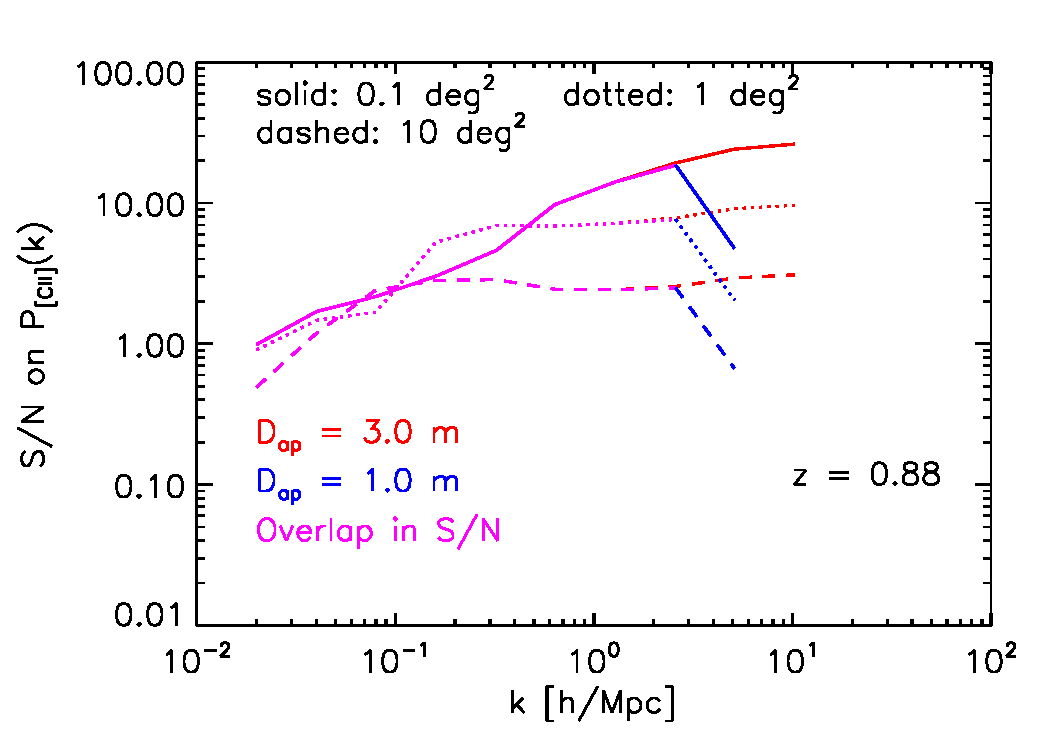
\includegraphics[width=0.4\textwidth]{snr_vs_k_ap3m_ap1m_asurveys_uhp_obs_z88_6dec2013} \\
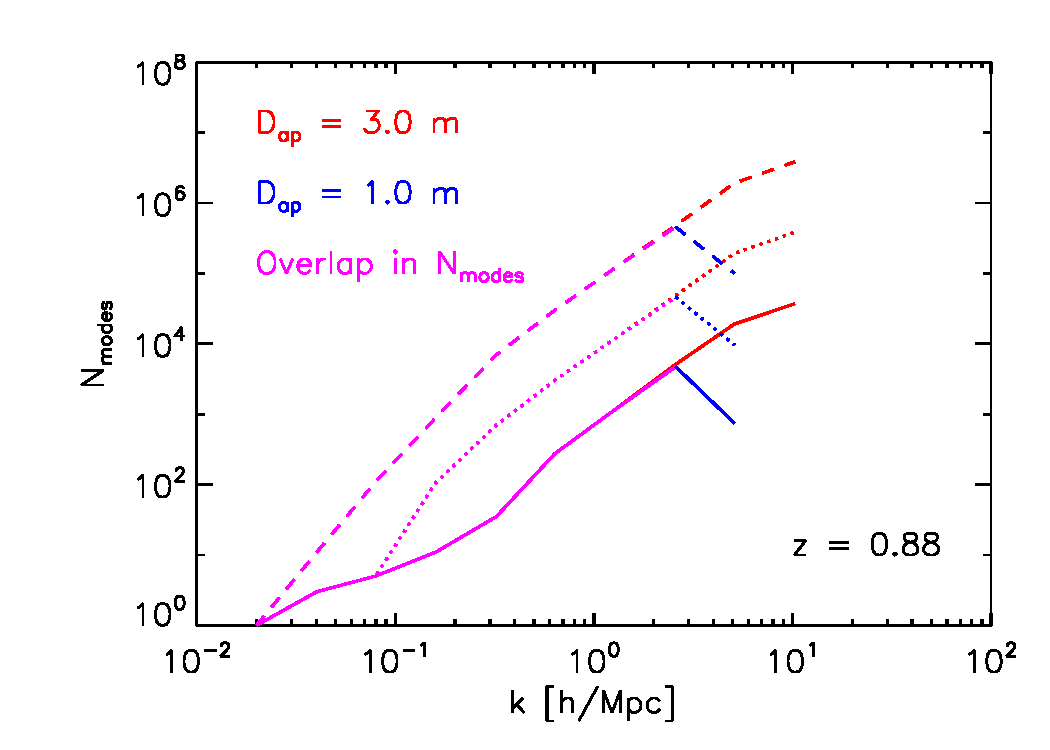
\includegraphics[width=0.4\textwidth]{nmode_vs_k_ap3m_ap1m_asurveys_uhp_obs_z88_6dec2013} \\
\end{tabular}
\caption{\label{} Signal to noise on the dimensionless [CII] power spectrum $\Delta_{\textrm{[CII], [CII]}}^2$ and number of modes as a function of $k$. The blue lines represent S/N for the 1 meter aperture, red denotes a 3 meter aperture, and purple shows where the two overlap. Survey areas of 0.1, 1, 10 square degree fields are shown as the solid, dashed, and dotted lines, respectively.}
\end{figure}

\section{Observational Strategy}

Now let us turn to a question regarding the motivation for intensity mapping in general, as well as in the specific case of [CII] at the redshifts relevant to this study. Having identified the galaxy redshift surveys as an alternative method to measure the 3D clustering power spectrum, it is natural to ask: In which regime does intensity mapping measure the power spectrum with higher SNR than the traditional galaxy surveys?

The expressions for SNR on a $k$ bin of interest for galaxy and intensity mapping surveys (denoted, respectively, by the subscripts ``GS" and ``IM") are

\begin{eqnarray}
\textrm{SNR}_{GS}  = \frac{\sqrt{N_{modes}} }{1 + 1/(P_{gal}\bar{n}_{gal} )} \\
\textrm{SNR}_{IM} =  \frac{\sqrt{N_{m}}}{1 + P_N/P_{line}}
\end{eqnarray}

To facilitate our comparisons in what follows, we employ toy models for the IR LF (Figure XX) written in the Schechter formalism---parametrized by the usual $\alpha$, $L_*$, and $\phi_*$---and normalize the total luminosity density to the empirical model from Section 2 (cf. Appendix for details). We stress that these Schechter models are not intended to represent a real interpretation of the distribution of galaxies, but are merely helpful for illustrating the effect of the LF \emph{shape} on the relative usefulness of intensity mapping and traditional galaxy surveys.
\begin{figure}
\centering
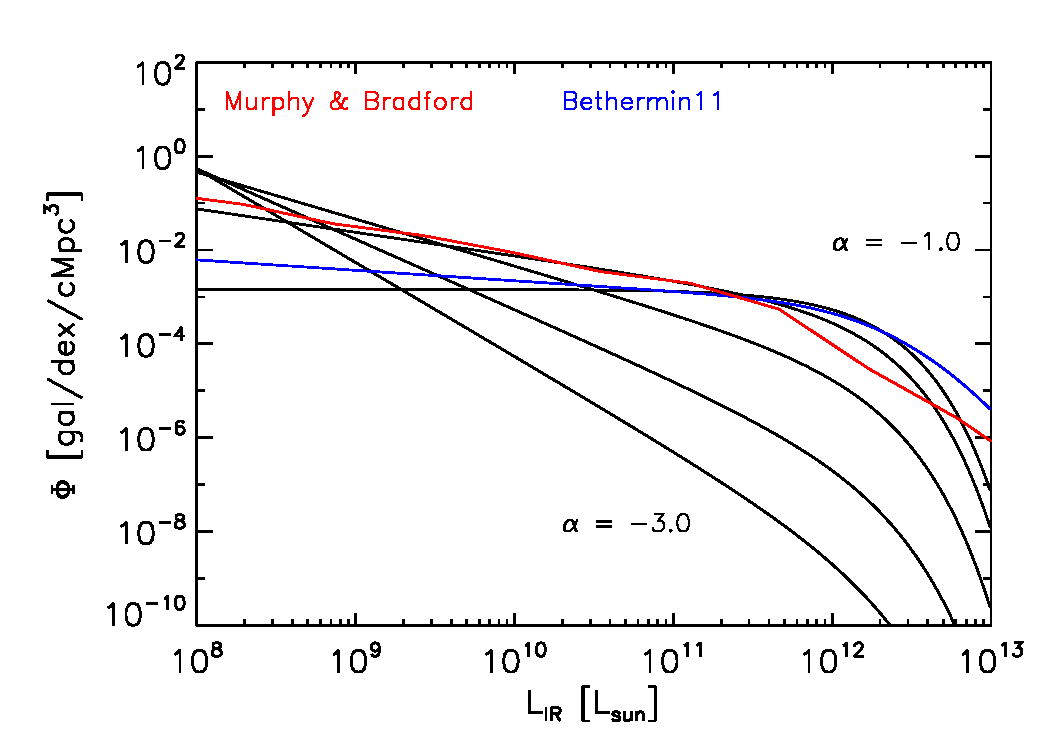
\includegraphics[width=0.4\textwidth]{phi_lir_schechter_bethermin11_murphy_Lstar1d12_Lmin1d8_Lmax1d13}
\caption{\label{} Luminosity Functions}
\end{figure}
The line sensitivity, $S_{\gamma}$ (units of W m$^2$ s$^{1/2}$), is the figure of merit for detecting an unresolved line in a point source, and we define individual detections at the $5\sigma$ level as having a flux above the instrumental noise in a pixel, i.e., above $5 \times S_{\gamma} t_{pix}^{-1/2}$. A convenient expression, which explicitly ties the minimum detectable luminosity to a broader framework of experimental variables, for the detection threshold can be written as
\begin{equation}
L_{i, min} = 5 \times f_{err}\rho_i V_{pix}, 
\end{equation}
Here, $f_{err}$ is the fractional error, 
\begin{equation}
f_{err} = \left(\frac{\sigma_N}{\sqrt{t_{pix}}}\right)/\bar{S}_i(z)
\end{equation}
 and $\rho_{i}(z)$ is the comoving luminosity density of line $i$ at some $z$, or $L_*\phi_* \Gamma(2+\alpha, L/L_*)$ in the Schechter notation, so that
\begin{equation}
\frac{L_{i,min}}{4\pi D_L^2} \Leftrightarrow 5 \times S_{\gamma} t_{pix}^{-1/2}
\end{equation}
 
Recall that the units of $\frac{\sigma_{N}}{\sqrt{t_{pix}}}$ and $S_{i}$ are Jy sr$^{-1}$, which does not depend on aperture. %One converts between $\sigma_N$ and $S_{\gamma}$ by dividing (or multiplying) by the frequency resolution d$\nu$ and beam solid angle d$\Omega$.
 \begin{figure}
\centering
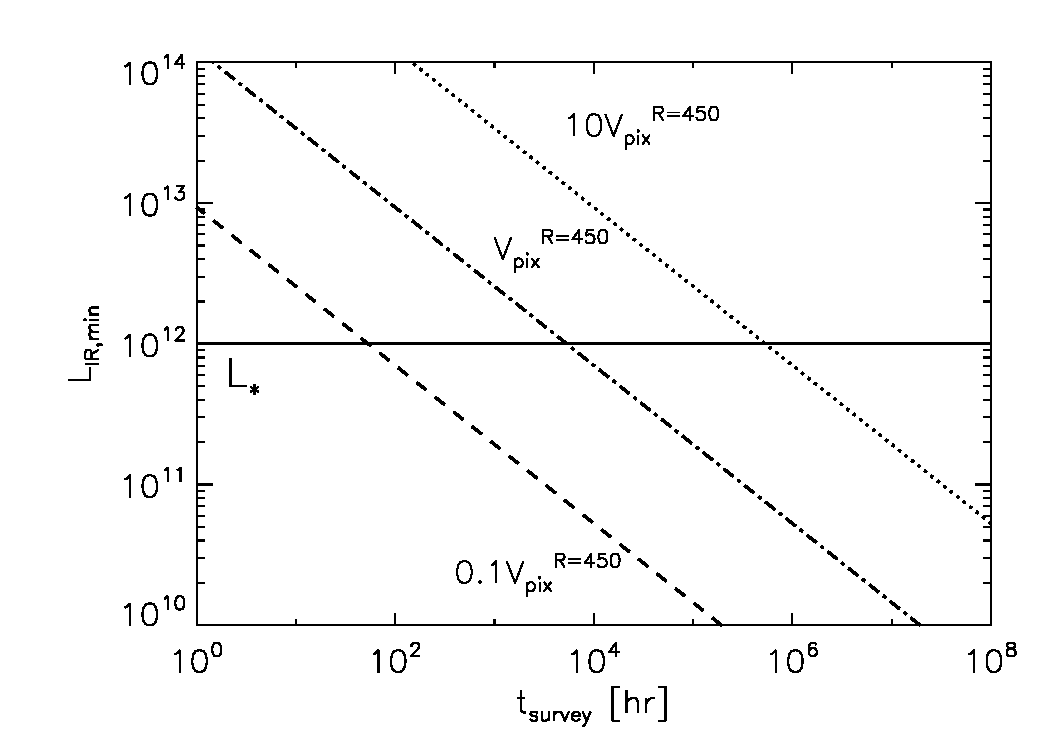
\includegraphics[width=0.4\textwidth]{lirmin_vs_tsurvey_lstar1d12_starfire_Vpix_0p1Vpix_10Vpix}
\caption{\label{} $L_{IR,min}$ as a function of the survey observing time, for various $V_{pix}$. The value of our adopted $L_{*}$ is plotted for comparison.}
\end{figure}
Written in this way, the detection threshold $L_{i,min}$ already provides some insight as to the optimal regimes for intensity mapping and galaxy surveys. Firstly, for $L_{i,min} \ll L_*$, we expect the galaxy surveys to be an effective means of studying the galaxy population, since the number of detections will be high and the shot noise term will be low. On the other hand, if $L_{i, min} \gg L_*$, then the galaxy survey will not be able to detect a significant fraction of galaxies that comprise the faint-end of the luminosity function, and intensity mapping becomes the ideal survey method, since it is sensitive to the total emission at a given redshift.

Now, suppose the voxels are increased in size by some factor $\alpha > 1$ due to a decrease in aperture diameter by $\sqrt{\alpha}$, but the survey area and survey observing time are left unchanged, leading to the following transformations on $t_{pix}$, the large scale clustering modes $N_{modes}^{clust}$, $P_{N}$, $f_{err}$, and, ultimately, $L_{i,min}

\begin{eqnarray}
t_{pix} \rightarrow t_{pix}^{\prime} &= \alpha t_{pix} \\
N_{modes}^{clust} \rightarrow N_{modes}^{clust \prime} &= N_{modes}^{clust} \\
P_N \rightarrow P_N^{\prime} &= P_{N} \\
f_{err} \rightarrow f_{err}^{\prime} &= \frac{f_{err}}{\sqrt{\alpha}} \\
L_{i,min} \rightarrow L_{i,min}^{\prime} &= \sqrt{\alpha} L_{i,min}
\end{eqnarray}

As a momentary detour on internal consistency, we note that an increase in aperture diameter by $\sqrt{\alpha}$ also results in an increase in the righthand side of Equation 15 by the same factor $\sqrt{\alpha}$ that appears in Equation 20 after applying the analogous transformations for the line sensitivity:

\begin{eqnarray}
S_{\gamma} \rightarrow S_{\gamma}^{\prime} = \alpha S_{\gamma}\\
t_{pix} \rightarrow t_{pix}^{\prime} = \alpha t_{pix} \\
\end{eqnarray}

Thus, the increase of $L_{i,min}$ with $V_{pix}$ suggests that traditional galaxy surveys with large voxels, such that $L_*\phi_* \Gamma(2+\alpha, L/L_*) V_{pix} \gg 1$, will find themselves in the disabling condition of having many sources that are below the detection threshold in a single voxel. On the other hand, because the intensity mapping method does not aim to detect individual galaxies, it will still be able to measure clustering in the large voxel limit with high SNR. Figure 6 is meant to demonstrate the small (top panel) and large (bottom panel) limits in the case of [CII] at $z = 1.5$. In this figure, survey area has been fixed at $A_{survey} = 5.3$ deg$^2$, and pixels have been conformally contracted (expanded) to 0.1$\times V_{pix}^{R=450}$ ($10\times V_{pix}^{R=450}$). According to Figure XX, the galaxy surveys do very well with the small pixels, as expected, since large telescopes with fine spectral resolution indeed follow the typical design of these experiments, but require large amounts of observing time (in excess of $10^4$ hr) to reach $\textrm{SNR}_{tot}^{clust} \sim 10$ in the large pixel limit. Notice that the SNR for the intensity mapping curve (in magenta) retains the same values as in Figure XX for a given total observing time---reaching $\textrm{SNR}_{tot}^{clust}$ \sim 10$ in roughly 1,000 hours---which is precisely the behavior we have seen when considering the relative performance of the telescopes with $D_{ap} = 1.0$ m and 3.0 m, which have approximately a factor of 10 difference in size of their respective diffraction limited beams. (Briefly, the number of clustering modes and $P_N$ are unscathed by an increase in beam size for a fixed survey area, so SNR is preserved.)

Another scenario in which an experiment finds itself in the large pixel limit is for observations at long wavelengths. Figure 6 shows the envisioned balloon-borne experiment performing a 5.3 deg$^{2}$ survey map of [CII] between $z = 5.4$ and $z = 6.6$, with central frequency now redshifted to 270 GHz (corresponding to $z = 6$) and spectral resolution maintained at $R=450$. (For direct comparison, the experiment at $z=1.5$ is plotted in Figure 7.) At these frequencies, we have extrapolated the NEI and line sensitivities to $3 \times 10^5$ Jy sr$^{-1}$ s$^{1/2}$ and $4.8\times10^{-19}$ W m$^{-2}$ s$^{1/2}$. As expected, in the large voxel limit, the relative performance of [CII] intensity mapping survey and the traditional galaxy surveys in measuring the galaxy clustering becomes even more disparate than at $z=1.5$, in favor of intensity mapping.

\begin{figure}[h]
 \centering
 \subfloat{
 \label{}
 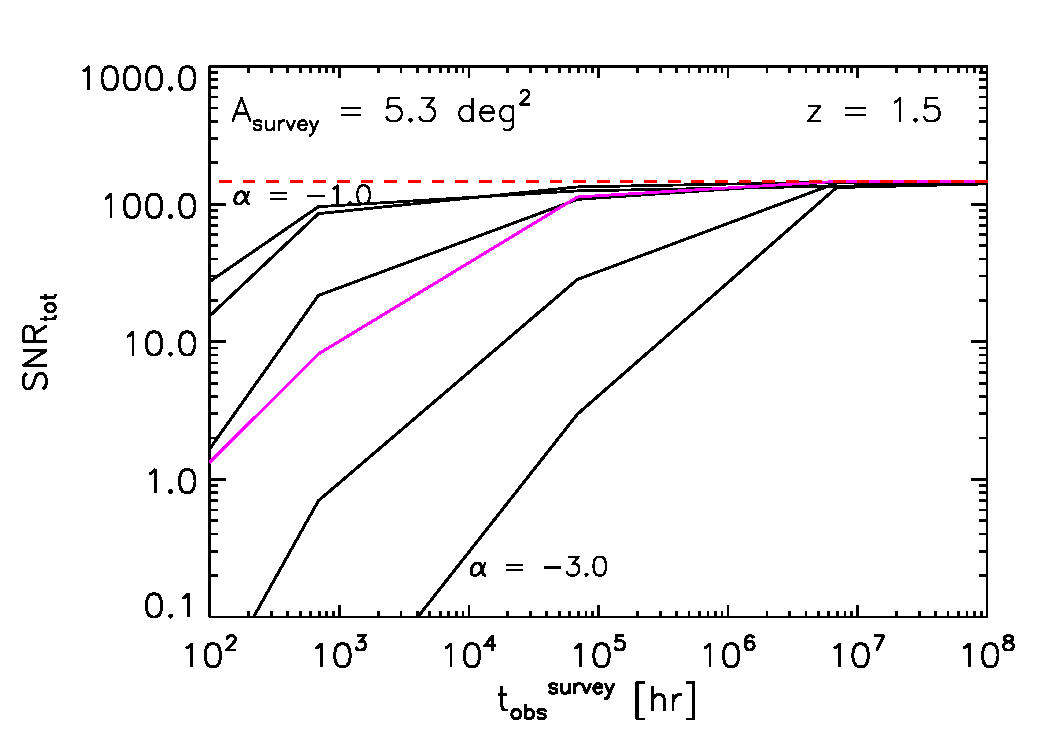
\includegraphics[width=0.4\textwidth]{SNRtot_starfire_cii_z1p5_ferr_beta_im_0p1VpixR450_Lstar1d12_Lmin1d8_Lmax1d13}}
 \subfloat{
 \label{fig:bethermin_fir_frac}
 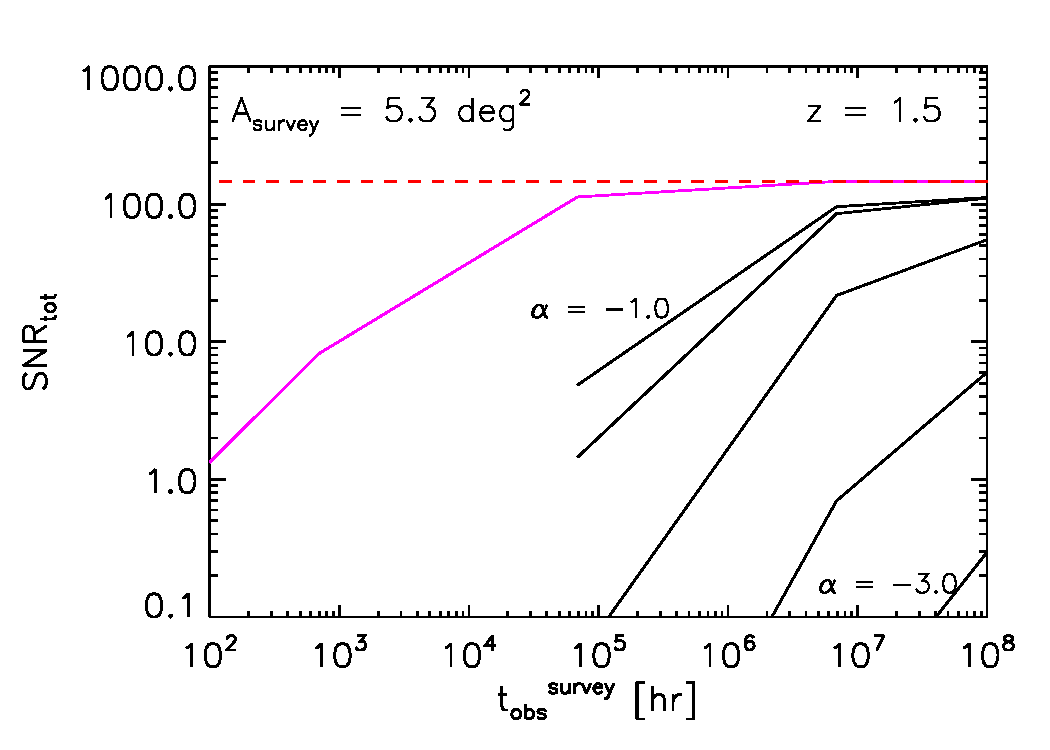
\includegraphics[width=0.4\textwidth]{SNRtot_starfire_cii_z1p5_ferr_beta_im_10VpixR450_Lstar1d12_Lmin1d8_Lmax1d13}}
 \centering
\caption{Total SNR on the clustering power spectrum as a function of survey time for the survey volume in Figure 3, for the intensity mapping and traditional galaxy survey methods, with pixel sizes $V_{pix} = 0.1\times$ and $10 \times V_{pix}^{R=450}$. Voxels have been contracted and expanded so as to preserve the ratios among the lengths of the sides.}
\end{figure}

\begin{figure}[h]
 \centering
 \subfloat{
 \label{}
 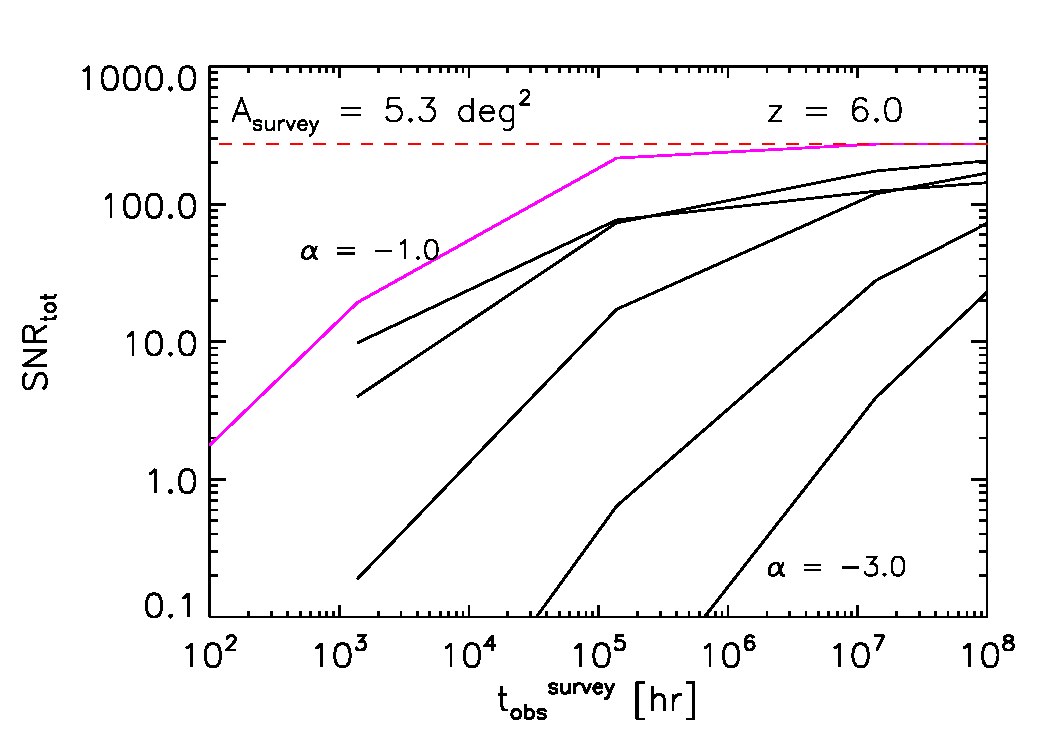
\includegraphics[width=0.4\textwidth]{SNRtot_starfire_cii_z1p5_ferr_beta_im_VpixR450_Lstar1d12_Lmin1d8_Lmax1d13_z6}}
 \subfloat{
 \label{fig:bethermin_fir_frac}
 \includegraphics[width=0.4\textwidth]{Ngal_cii_STARFIRE_5p3sqdeg_z6_ferr}}
 \centering
\caption{Same as Figure XX, but for $z = 6.0$}
\end{figure}


\begin{figure}[h]
 \centering
 \subfloat{
 \label{}
 \includegraphics[width=0.4\textwidth]{SNRtot_starfire_cii_z1p5_ferr_beta_im_VpixR450_Lstar1d12_Lmin1d8_Lmax1d13}}
 \subfloat{
 \label{fig:bethermin_fir_frac}
 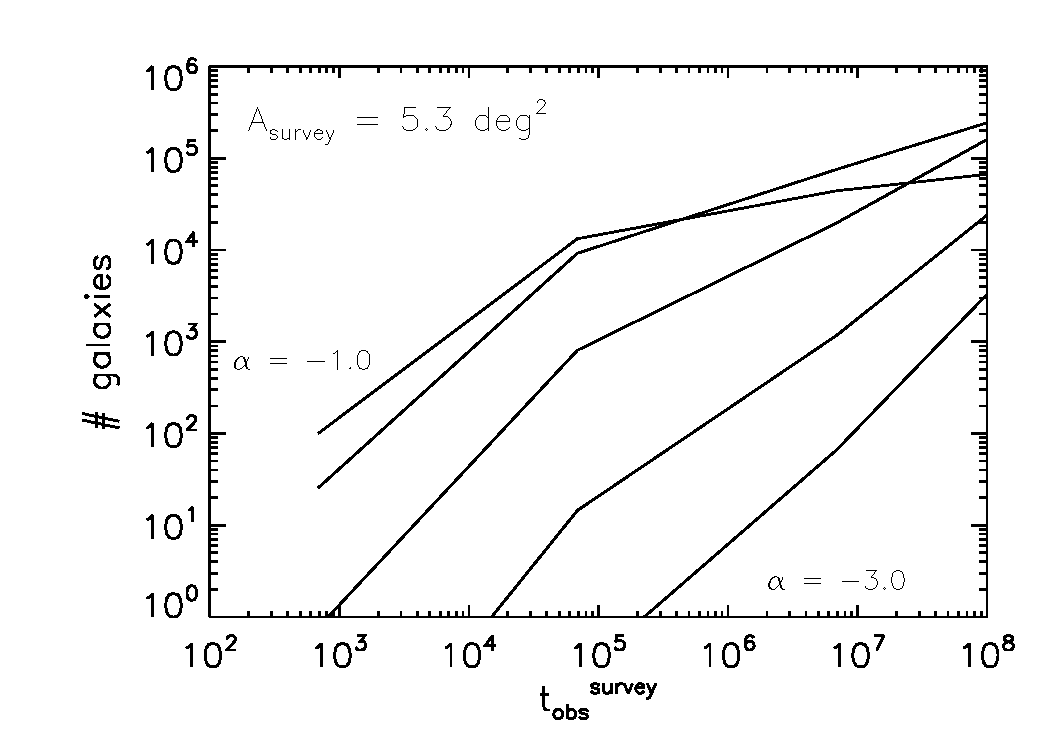
\includegraphics[width=0.4\textwidth]{Ngal_cii_STARFIRE_5p3sqdeg_z1p5_ferr}}
 \centering
\caption{Top panel: Total Signal-to-Noise ratio ($\textrm{SNR}_{tot}$) on the clustering power spectrum of [CII] at $z=1.5$ as a function of the survey observing time (in hours). $\textrm{SNR}_{tot}$ as computed from intensity mapping---which depends only on the integral of the luminosity function, and not the shape---and from the Schechter function models are plotted as magenta and black curves, respectively. The Schechter function models are plotted with slope decreasing from top to bottom. The horizontal dashed \emph{red line} is the maximum SNR, set by the number of modes in the survey volume. Bottom panel: Number of detectable galaxies in the 5.3 deg$^2$ survey as a function of total observing time according to the Schechter function models.}
\end{figure}




\bibliography{master_references}

\end{document}







